\documentclass[presentation]{beamer}


%width is width of sidebar
\usetheme{Madrid}

%school logo here
\logo{\includegraphics[height=1cm]{logo_vertical.pdf}\vspace{1pt}}


\usepackage{amsmath, mathtools}
\usepackage{amsfonts}
\usepackage{amsthm}
\usepackage{amssymb}
\usepackage{dsfont}
\usepackage{graphicx}
\usepackage{tikz}
\usetikzlibrary{arrows.meta}

\usefonttheme{serif}

\title{Caracterización de cuerpos finitos}
\author{Kevin Velez}
\institute{Universidad del Valle}
\date{Febrero 7, 2023}

\newcommand{\F}{\mathds{F}}
\newcommand{\Z}{\mathds{Z}}
\newcommand{\K}{\mathds{K}}

\begin{document}
\section{Caracterización de cuerpos finitos}
\begin{frame}
\maketitle
\end{frame}

\begin{frame}{Caracterización de cuerpos finitos}
  \begin{block}{Ejemplos conocidos de cuerpos finitos}
    \begin{equation*}
      \F_p = \Z / p\Z
    \end{equation*}
    Es un cuerpo finito con $p$ elementos para todo $p$ primo.
  \end{block}
\end{frame}

\begin{frame}
  \begin{block}{Lema 1}
    Sea $F$ un cuerpo finito conteniendo un subcuerpo $K$ con $q$ elementos. Entonces $F$ tiene $q^m$ elementos, donde $ m = [F : K] $ 

    \begin{figure}[H]
      \centering
      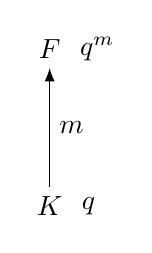
\begin{tikzpicture}
        \node (F) at (0,2) {$F$} node (K) at (0,0) {$K$}; 
        \draw[{Latex}-] (F) -- (K);
        \node[right] at (K.east) {$q$};
        \node[right] at (F.east) {$q^m$};
        \node[right] at (0,1) {$m$};
      \end{tikzpicture}
    \end{figure}
  \end{block}
\end{frame}


\begin{frame}
  \begin{block}{Teorema 2}
    Sea $F$ un cuerpo finito, entonces $F$ tiene $p^n$ elementos, donde el primo $p$ es la característica de $F$ y $n$ es el grado de $F$ sobre su cuerpo primo.

    \begin{figure}[H]
      \centering
      \begin{tikzpicture}
        \node (F) at (0,2) {$F$} node (F') at (0,0) {$F'$}; 
        \draw[{Latex}-] (F) -- (F');
        \node[right] at (0,1) {$n$};
        \node at (3,1) {\small $\mbox{ch}(F) = p$};
        \node at (-3,1) {};
      \end{tikzpicture}
    \end{figure}
  \end{block}
\end{frame}

\begin{frame}
  \begin{block}{Construcción de nuevos cuerpos finitos}
    Si $f \in \F_p[x]$ es un polinomio irreducible de grado $n$, entonces $\F_p[x]/(f)$ es un cuerpo finito de $p^n$ elementos.

    \vspace{2em}
    ¿Siempre es posible encontrar un polinomio irreducible en $\F_p$ de grado $n$ para todo entero positivo $n$?
  \end{block}
\end{frame}

\begin{frame}
  \begin{block}{Lema 3}
    Si $F$ es un cuerpo finito con $q$ elementos, entonces cada $a \in F$ satisface $a^q = a$.
  \end{block}
  \pause
  \begin{block}{Lema 4}
    Si $F$ es un cuerpo finito con $q$ elementos, y $K$ es un subcuerpo de $F$, entonces el polinomio $x^q - x \in K[x]$ se factoriza en $F[x]$ como 
    \begin{equation*}
      x^q - x = \prod_{a \in F} (x - a)
    \end{equation*}
    y $F$ es un cuerpo de descomposición de $x^q - x$ sobre $K$.
  \end{block}
\end{frame}

\begin{frame}
  \begin{block}{Teorema 5 (Existencia y unicidad de cuerpos finitos)}
    Para cada primo $p$ y cada entero positivo $n$, existe un cuerpo finito con $p^n$ elementos. Cualquier cuerpo con $q = p^n$ elementos es isomorfo al cuerpo de descomposición de $x^q - x$ sobre $\F_p$.
  \end{block}
  \pause
  \begin{block}{Cuerpos de Galois}
    Ahora, podemos hablar de cuerpos finitos o cuerpos de Galois de orden $q$, denotados $\F_q$, donde $q=p^n$ con $p$ primo.
  \end{block}
\end{frame}

\begin{frame}
  \begin{block}{Ejemplos}
    \begin{itemize}
      \item Consideremos $f(x) =   x^2 + x + 2 \in \F_3[x]$, el cual es un polinomio irreducible de grado $2$ sobre $\F_3$. Sea $\theta$ una raíz de $f(x)$ en algún cuerpo. Construimos entonces el cuerpo $\F_3(\theta) = \left\{a + b\theta: a,b \in \F_3 \right\}$ un cuerpo con $9$ elementos, y entonces $\F_3(\theta) = \F_9$.
      \pause
      \item Del mismo modo, consideremos $f(x) = x^2 + x + 1 \in \F_2[X]$ irreducible, y $\theta$ una raíz, entonces $\F_2(\theta) = \F_4$.
    \end{itemize}
  \end{block}
\end{frame}

\begin{frame}
  \begin{block}{Teorema 6 (Criterio de subcuerpos)}
    Sea $\F_q$ un cuerpo finito con $q=p^n$ elementos. Entonces cada subcuerpo de $\F_q$ tiene orden $p^m$ donde $m$ es un divisor positivo de $n$. Recíprocamente, si $m$ es un divisor positivo de $n$, entonces hay exactamente un subcuerpo de $\F_q$ con $p^m$ elementos.

    \begin{figure}[H]
      \centering
      \begin{tikzpicture}
        \node (F) at (0,2) {$\F_{p^n}$} node (K) at (0,0) {$F_{p^m}$}; 
        \draw[{Latex}-] (F) -- (K);
        \node[right] at (0,1) {$\frac{n}{m}$};
        \node at (3,1) {$m$ divisor de $n$};
        \node at (-3,1) {};
      \end{tikzpicture}
    \end{figure}
  \end{block}
  \pause
  \begin{block}{Observación}
    El único subcuerpo de $\F_{p^n}$ de orden $p^m$ donde $m$ es un divisor positivo de $n$, consiste de las raíces del polinomio $x^{p^m}-x \in \F_p[x]$ en $\F_{p^n}$.
  \end{block}
\end{frame}

\begin{frame}
  \begin{block}{Ejemplo 7}
    Los subcuerpos del cuerpo finito $\F_{2^30}$ pueden ser determinados listando todos los posibles divisores positivos de $30$. La relación de contenencia entre estos subcuerpos es equivalente a la relación de divisibilidad entre los divisores de $30$.

    \begin{figure}[H]
      \centering
      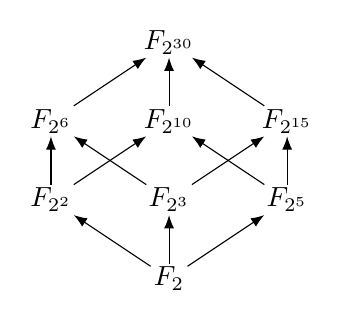
\begin{tikzpicture}
        \begin{scope}[inner sep=1pt, -{Latex}]
          \node (F30) at (0,3) {$\F_{2^{30}}$};
          
          \node (F6) at (-1.5,2) {$\F_{2^{6}}$};
          \node (F10) at (0,2) {$\F_{2^{10}}$};
          \node (F15) at (1.5,2) {$\F_{2^{15}}$};
          
          \node (F2) at (-1.5,1) {$\F_{2^{2}}$};
          \node (F3) at (0,1) {$\F_{2^{3}}$};
          \node (F5) at (1.5,1) {$\F_{2^{5}}$};
          
          \node (F1) at (0,0) {$\F_{2}$};

          \draw (F1) -- (F2);
          \draw (F1) -- (F3);
          \draw (F1) -- (F5);

          \draw (F2) -- (F6);
          \draw (F2) -- (F10);

          \draw (F3) -- (F6);
          \draw (F3) -- (F15);

          \draw (F5) -- (F10);
          \draw (F5) -- (F15);

          \draw (F6) -- (F30);

          \draw (F10) -- (F30);

          \draw (F15) -- (F30);
        \end{scope}
      \end{tikzpicture}
    \end{figure}
  \end{block}
\end{frame}

\begin{frame}
  \begin{block}{Teorema 8}
    para cada cuerpo finito $\F_q$, el grupo multiplicativo $ {\F_{q}}^* $ de elementos no cero de $\F_q$ es cíclico.
  \end{block}
  \pause
  \begin{block}{Definición 9}
    Un generador del grupo cíclico ${\F_q}^*$ es llamado un elemento primitivo de $\F_q$.
  \end{block}
  \pause
  $ {\F_q}^* $ tiene $\phi(q-1)$ elementos primitivos.
\end{frame}

\begin{frame}
  \begin{block}{Ejemplo}
    \begin{itemize}
      \item $\F_5$ tiene $\phi(4) = 2$ elementos primitivos, estos son $2$ y $3$.
      \pause
      \item $\F_4$ tiene $\phi(3) = 2$ elementos primitivos. Expresando $\F_4$ como $\F_2(\theta) = \{0, 1, \theta, \theta + 1\}$, donde $\theta^2 + \theta + 1 = 0$, encontramos que $\theta$ y $\theta + 1$ son los elementos primitivos de $\F_4$.
    \end{itemize}
  \end{block}
\end{frame}

\begin{frame}
  \begin{block}{Teorema 10}
    Sea $\F_q$ un cuerpo finito y $\F_r$ una extensión finita. Entonces $\F_r$ es una extensión algebraica simple de $\F_q$.
    
    \begin{figure}[H]
      \centering
      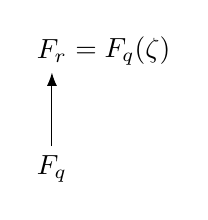
\begin{tikzpicture}
        \node (Fr) at (0,1.5) {$\F_r$};
        \node (Fq) at (0,0) {$\F_q$};
        \draw[-{Latex}] (Fq) -- (Fr);
        \node[right, xshift=-4pt] at (Fr.east) {$= \F_q(\zeta)$};
      \end{tikzpicture}
    \end{figure}
  \end{block}
  \pause 
  \begin{block}{Corolario 11}
    Para cada cuerpo finito $\F_q$ y cada entero positivo $n$, existe un polinomio irreducible $ \F_q[x]$ de grado $n$.
  \end{block}
\end{frame}

\begin{frame}
  \begin{block}{Ejemplo}
    Consideremos el cuerpo finito $\F_9$, lo podemos expresar en la forma $\F_3(\beta)$, donde $\beta$ es una raíz del polinomio $x^2+1$, irreducible sobre $\F_3$,. Sin embargo, como $\beta^4 = 1$, $\beta$ no es un generador de ${\F_9}^*$. Por lo tanto, $\beta$ no es un elemento primitivo de $\F_9$.
  \end{block}
\end{frame}

\section{Raíces de polinomios irreducibles}

\begin{frame}{Raíces de polinomios irredubles sobre cuerpos finitos}
  \begin{block}{Lema 12}
    Sea $f \in \F_q[x]$ un polinomio irreducible sobre un cuerpo finito $\F_q$ y sea $\alpha$ una raíz de $f$ es una extensión de cuerpo de $\F_q$. Entonces para un polinomio $h \in \F_q[x]$ tenemos que $h(\alpha) = 0$ si y solo si $f$ divide a $h$.
  \end{block}
  \pause
  \begin{block}{Lema 13}
    Sea $f \in \F_q[x]$ un polinomio irreducible sobre $\F_q$ de grado $m$. Entonces $f(x)$ divide a $x^{q^m}-x$ si y solo si $m$ divide a $n$.
  \end{block}
\end{frame}

\begin{frame}
  \begin{block}{Teorema 14}
    Si $f$ es un polinomio irreducible en $\F_q[x]$ de grado $m$, entonces $f$ tiene una raíz $\alpha$ en $\F_{q^m}$. Más aún, todas las raíces de $f$ son simples y están dadas por los $m$ distintos elementos $\alpha, \alpha^q, \alpha^{q^2}, \ldots, \alpha^{q^{m-1}}$ de $\F_{q^m}$.
  \end{block}
  \pause
  \begin{block}{Corolario 15}
    Sea $f$ un polinomio irreducible en $\F_q[x]$ de grado $m$. Entonces el cuerpo de descomposición de $f$ sobre $\F_q$ es $\F_{q^m}$.
  \end{block}
  \pause 
  \begin{block}{Corolario 16}
    Cualesquier dos polinomios irreducibles en $\F_q[x]$ del mismo grado tienen cuerpos de descomposición isomorfos.
  \end{block}
\end{frame}

\begin{frame}
  \begin{block}{Definición 17}
    Sea $\F_{q^m}$ una extensión de $\F_q$ y sea $\alpha \in \F_{q^m}$, entonces los elementos $\alpha, \alpha^q, \alpha^{q^2}, \ldots, \alpha^{q^{m-1}}$ son llamados conjugados de $\alpha$ respecto a $\F_q$.
  \end{block}
  \pause
  Los conjugados de $\alpha \in \F_{q^m}$ con respecto a $\F_q$ son distintos si y solo si el polinomio minimal de $\alpha$ en $\F_q[x]$ es de grado $m$. En otro caso, el grado $d$ de este polinomio minimal es un divisor propio de $m$ y los conjugados de $\alpha$ con respecto a $\F_q$ son los elementos $\alpha, \alpha^q, \alpha^{q^2}, \ldots, \alpha^{q^{d-1}}$. repetidos cada uno $\frac{m}{d}$ veces.
\end{frame}

\begin{frame}
  \begin{block}{Teorema 18}
    Los conjugados de $\alpha \in {\F_q}^*$ con respecto a cualquier subcuerpo de $\F_q$ tienen el mismo orden en el grupo ${\F_q}^* = \langle \zeta \rangle$
  \end{block}
  \pause
  \begin{block}{Corolario 19}
    Si $\alpha$ es un elemento primitivo de $\F_q$, entonces también lo son todos sus conjugados con respecto a cualquier subcuerpo de $\F_q$.
  \end{block}
\end{frame}

\begin{frame}
  \begin{block}{Ejemplo 20}
    Sea $\alpha \in \F_{16}$ una raíz de $f(x) = x^4 + x + 1 \in \F_2[x]$. Entonces los conjugados de $\alpha$ respecto a $\F_2$ son $\alpha, \alpha^2, \alpha^4 = \alpha+1$ y $\alpha^8 = \alpha^2 + 1$. Siendo cada uno de ellos un elemento primitivo de $\F_{16}$.

    \vspace*{1em}
    Los conjugados de $\alpha$ respecto a $\F_4$ son $\alpha$ y  $\alpha^4 = \alpha+1$.
  \end{block}
\end{frame}

\begin{frame}
  \begin{block}{Teorema 21}
    Los distintos automorfismos de $\F_{q^m}$ sobre $\F_q$ son exactamente los automorfismos $\sigma_0, \sigma_1, \ldots, \sigma_{m-1}$ definidos por $\sigma_j (\alpha) = \alpha^{q^j}$ con $\alpha \in \F_{q^m}$ y $0 \leq j \leq m-1 $. Estos automorfismos son reciben el nombre de \emph{Automorfismos de Frobenius}
  \end{block}
\end{frame}

\begin{frame}
  \begin{block}{}
    Con base en el teorema 21, resulta evidente que los conjugados de $\alpha \in \F_{q^m}$ con respecto a $\F_q$ son obtenidos mediante la aplicación de todos los automorfismos de $\F_{q^m}$ sobre $\F_q$ al elemento $\alpha$.
  \end{block}

  \begin{block}{}
    Los automorfismos de $F_{q^m}$ sobre $\F_q$ forman un grupo con la operación usual de composición. Por el teorema 21, este grupos es cíclico de orden $m$, generado por $\sigma_1$.
  \end{block}

  \begin{block}{}
    Como $[\F_{q^m}:\F_q] = m$, entonces $\F_{q^m}$ es de Galois sobre $\F_q$, entonces
    \begin{equation*}
      \mbox{Gal}(\F_{q^m} / \F_q) = \langle \sigma_1 \rangle \cong \Z / m\Z
    \end{equation*}
  \end{block}
\end{frame}

\begin{frame}
  \begin{block}{Referencias}
    \nocite{*}
    \bibliographystyle{plain}
    \bibliography{referencias}
  \end{block}
\end{frame}
\end{document}
